%	VERSIONE 0.2

\documentclass[a4paper,twocolumn,notitlepage]{book}
\usepackage[T1]{fontenc}
\usepackage[utf8]{inputenc}
\usepackage{lmodern}
\usepackage[italian]{babel}
\usepackage{indentfirst}
\usepackage{graphicx}
\usepackage{amsmath}
\usepackage{booktabs}
\usepackage{microtype}

\pagestyle{plain}

\begin{document}
	\onecolumn
	\title{Appunti di Fondamenti di Elettronica}
	\maketitle	
	\section*{Introduzione}
	L'esame di Fondamenti di Elettronica richiede precisione non tanto sui calcoli ma sulle considerazioni da fare.
	Oltre allo svolgimento dei calcoli, è quindi necessario scrivere e spiegare tutto quello che si fa; questo purtroppo porta ad avere poco tempo per eseguire il compito.

	Per il resto, dal punto di vista matematico i calcoli da eseguire non vanno oltre l'algebra elementare, 
	mentre è richiesta una conoscenza discreta di Elettrotecnica (legge di Ohm, principi di Kirchhoff per correnti e tensioni, partitore di tensione, circuiti equivalenti di Thévenin, specialmente con generatori pilotati) e una conoscenza base di Analisi dei Sistemi/Controlli Automatici (risposta in frequenza, pulsazione di taglio a -3 dB, pulsazione di attraversamento, poli-zeri, funzione di trasferimento). Può essere d'aiuto utilizzare una calcolatrice in grado di risolvere equazioni di secondo grado, perché permette di risparmiare tempo nel calcolo del punto di riposo.
	\newpage
	\twocolumn
	
	\section*{Amplificatori a MOSFET}
		\subsection*{Considerazioni Preliminari}	
			Come sapete bene, nello studio degli amplificatori a MOSFET è di fondamentale importanza l'analisi "a piccolo segnale", per studiarne alcuni dei suoi parametri fondamentali. 
Per farlo sono neccessarie delle solide basi in elettrotecnica (circuiti equivalenti di Thévenin e Norton), che in questo breve documento daremo per scontate. A dirla tutta, non affronteremo l'analisi a piccolo segnale in grande dettaglio: è già spiegata in modo più che esaustivo in qualunque libro di Elettronica. 
È sufficiente dire che al circuito di partenza ne va sostituito uno fatto in questo modo: le alimentazioni diventano collegamenti a massa, i capacitori cortocircuiti, il MOSFET da un generatore di corrente $i_{d}$ controllato da $v_{gs}$ con transconduttanza $g_{m}$,

\begin{equation}
	i_{d}=g_{m}v_{gs}
\end{equation}

Ovviamente non può pasare nessuna corrente attraverso il gate e questo viene modellato con un circuito aperto (impedenza infinita) tra gate-drain e gate-source.

**(medgives, qui mi avventuro in una pseudo-spiegazione, dimmi se secondo te ha senso)**

Il punto di tutto questo è che noi facciamo l'ipotesi di essere già in saturazione e a frequenze intermedie (concetti che verranno approfonditi in seguito), per questo non ci importa di alimentazione e capacitori. Noi vogliamo solo vedere cosa succede se applichiamo un segnale abbastanza piccolo da non modificare le condizioni di riposo.

		\subsection*{Stadi Elementari}
		
		\begin{itemize}
				\item \textbf{Common Source}
				\item \textbf{Common Gate}
				\item \textbf{Common Drain}
		\end{itemize}
			
		\subsection*{Massima escursione del segnale in uscita}
		La massima escursione del segnale in uscita da un amplificatore realizzato con un singolo MOSFET è limitata dalla possibilità che il componente esca dalla regione di saturazione, entrando quindi in interdizione o in regione di triodo.
		\begin{itemize}
			\item \textbf{Common Source} \newline
				Per non far entrare il transistor in regione di triodo, la $V_{DS}$ deve valere almeno la $V_{OV}$ di polarizzazione. Quindi un limite sull'escursione dell'uscita è dato da:
				\begin{equation}
					v_{o_{max}}=V_{DS}-V_{OV}
				\end{equation}				
				
				Per evitare l'interdizione del MOSFET devo fare in modo che sulle resistenze nel ramo drain-source scorra corrente. Saltando i calcoli, ciò si traduce nella seguente relazione:
				
				\begin{equation}
					v_{o_{max}}=I_D R_D
				\end{equation}
				
				La massima escursione di tensione in uscita è la più piccola delle due trovate.
			\item \textbf{Common Gate}  \newline
				Per evitare la regione di triodo:
				\begin{equation}
					v_{o_{max}}=V_{DS}-V_{OV}
				\end{equation}
				
				mentre per evitare l'interdizione:
				\begin{equation}
					v_{o_{max}}=I_D R_D
				\end{equation}
				
			\item \textbf{Common Drain}  \newline
				Per evitare la regione di triodo:
				\begin{equation}
					v_{o_{max}}=V_{DS}-V_{OV}
				\end{equation}
				
				mentre per evitare l'interdizione:
				\begin{equation}
					v_{o_{max}}=I_D R_S
				\end{equation}
		\end{itemize}
		È da notare come in un amplificatore a più stadi sia necessario valutare anche le tensioni intermedie in uscita e il guadagno dell'ultimo stadio. Esempio: in un amplificatore a due stadi potrei trovare che il primo ammette $V_{o_{max1}}=3V$, mentre il secondo $V_{o_{max2}}=2.9V$; inoltre il guadagno dell'ultimo stadio $A_{2}=0.9V/V$. In questo caso si potrebbe concludere affrettatamente che il secondo stadio impone il limite più basso, ma non deve sfuggire che $V_{o_{max1}}*A_{2}=2.7V < V_{o_{max2}}$. Quindi in effetti la massima escursione sarebbe di 2.7V.
	\subsection*{Massima escursione del segnale in ingresso}
	Una volta calcolata la massima escursione del segnale in uscita, è facile calcolare la massima escursione che può avere il segnale in ingresso.
	
	Se indichiamo con $A$ il guadagno dell'amplificatore, allora il segnale in uscita sarà:
	\begin{align*}
		V_{out}= A \cdot V_{in}
	\end{align*}		
	, perciò se conosciamo il valore massimo che può assumere $V_{out}$, il valore massimo del segnale in ingresso è facilmente calcolabile come:
	\begin{equation}
		V_{in_{max}}=\frac{V_{out_{max}}}{A}
	\end{equation}
	
	\subsection*{Calcolo del punto di riposo}
	In generale, per calcolare il punto di riposo Q di un MOSFET, è possibile seguire i seguenti passi:
	\begin{enumerate}
		\item
		Si aprono tutti i condensatori, perché lavoreremo in continua, ed essi in DC sono equivalenti a dei circuiti aperti;
		\item
		Si assume che il transistor lavori nella zona di saturazione, ovvero che $V_{DS} >= V_{OV}$. Questo passo è importante e va assolutamente scritto durante l'esame;
		\item
		Si applica la KVL alla maglia Gate-Source, per trovare la $V_{GS}$;
		\item
		Si utilizza il valore di $V_{GS}$ trovato per calcolare la corrente $I_D$. La formula da utilizzare è quella per il MOSFET in saturazione.\newline
		Inizialmente il calcolo viene fatto senza tener conto del parametro $\lambda$ (modulazione della lunghezza del canale); successivamente, quando si avrà anche una prima stima di $V_{DS}$, si dovrà tornare indietro per verificare se il risultato ottenuto tenendo conto di $\lambda$ stia entro la tolleranza delle resistenze;
		\item
		Si applica la KVL alla maglia Drain-Source e si usa il valore di $I_D$ per calcolare $V_{DS}$;
		\item
		Si verifica la veridicità dell'ipotesi di saturazione ($V_{DS} >= V_{OV}$). Se non è verificata, torna indietro e assumi un'altra regione di lavoro (altamente improbabile; la maggior parte delle volte è indice di errori concettuali o di calcolo);
		\item
		Si verifica lo scostamento di $I_{D}$ con l'introduzione del parametro $\lambda$. Se l'errore introdotto ($|I_{D (nuova)} - I_{D (vecchia)}|$) rientra nella percentuale di tolleranza delle resistenze che è data, allora va bene e possiamo tenere i nostri risultati.\newline
		Se non rientra, dobbiamo rifare i conti con l'introduzione del parametro $\lambda$ (cosa possibile nell'esame).
		\item
		Il punto di riposo $Q$ è dato dall'insieme dei parametri $I_D$, $V_{GS}$ e $V_{DS}$.		
		
	\end{enumerate}\medskip
	\textbf{NOTA:} Se $V_{DS}=V_{GS}$, ovvero drain e gate sono cortocircuitati, allora il transistor lavora certamente in saturazione, infatti $V_{DS} > V_{GS} - V_{th}$. Questo impone una scarsa escursione del segnale in uscita, che sarà limitato nella gran parte dei casi dalla $V_{th}$ stessa.
	
	Se la polarizzazione è ``a quattro resistenze'', $V_G$ è ottenuta tramite il partitore.
	
	\subsection*{Calcolo della frequenza di taglio inferiore $f_L$}
	Per il calcolo della frequenza di taglio inferiore, utilizziamo il metodo delle costanti di tempo in cortocircuito (SCTC, Short Circuit Time Constants). È necessario scrivere che si sta usando tale metodo, pena perdita di punteggio.\newline
	Il metodo è meccanico e permette di avere una buona stima. È necessario saper calcolare la resistenza di Thévenin con generatori pilotati. I passi sono i seguenti:
	\begin{enumerate}
		\item apro i condensatori uno per volta; gli altri condensatori sono sostituiti da cortocircuiti;
		\item sostituisco al MOSFET il modello a piccolo segnale;
		\item calcolo la resistenza equivalente vista ai capi del condensatore precedentemente aperto;
		\item per ogni condensatore avrò una costante di tempo $\tau_i=R_i C_i$;
		\item la frequenza di taglio inferiore sarà data da:
			\begin{equation}
				f_L=\frac{1}{2 \pi} \sum_{i=1}^n \frac{1}{\tau_i} \:=\: \frac{1}{2 \pi} \sum_{i=1}^n \frac{1}{R_i C_i}
			\end{equation}
	\end{enumerate}
	
	\section*{Amplificatori multistadio}
	\subsection*{Identificazione degli stadi elementari}
		\subsubsection*{Stadi a singolo transistor}	
		Per identificare gli stadi elementari a MOSFET (common source, common drain, common gate) basta seguire il percorso del segnale: se esso entra in un morsetto ed esce da un altro morsetto, il morsetto rimanente è detto  ``comune''  (common).
		Quindi, ad esempio, se il segnale entra nel gate ed esce dal source, allora lo stadio è un common drain.
	Per essere precisi, è meglio spendere anche due parole sulla alimentazione. 
Se essa è fornita tramite una sola tensione e massa, allora l'alimentazione è detta unipolare positiva o negativa, a seconda del segno della tensione.  \newline
		Se l'alimentazione è fornita tramite due tensioni di segno opposto e massa, essa è detta bipolare. Se le tensioni di segno opposto sono uguali, l'alimentazione è bipolare simmetrica, mentre è bipolare asimmetrica se sono diverse.
		\newline
		Esempio: \medskip
		
		\begin{tabular}{|c|c|}
		\hline
		\textbf{Caso} & \textbf{Tipo alimentazione} \\
		\hline
		+15V e massa & unipolare positiva \\
		-15V e massa & unipolare negativa \\
		+15V, -15V e massa & bipolare simmetrica \\
		+15V, -6V e massa & bipolare asimmetrica \\
		\hline
		\end{tabular}
		
		\subsubsection*{Stadi con amplificatore operazionale}
		Gli stadi con amplificatore operazionale possibili sono quattro: amplificatore invertente, amplificatore non invertente, filtro passa-basso, filtro passa-banda.
		\begin{itemize}
			\item \textbf{Amplificatore invertente e non invertente}\newline
				Se il segnale è applicato al morsetto invertente (segno -), l'amplificatore è invertente, altrimenti è non invertente.
				
				È da specificare che per la natura costruttiva dell'operazionale, queste due configurazioni hanno sempre un comportamento da filtro, normalmente passa-basso ma inserendo una capacità di blocco in ingresso si possono trasformare in passa-banda (su questo saranno necessarie altre specificazioni).
			\item \textbf{Filtro passa-basso attivo invertente}\newline
			Se nel ramo di retroazione è presente un condensatore in parallelo a una resistenza, lo stadio è un filtro passa-basso attivo.
			Si può vedere anche come un circuito integratore reale.
			
			\item \textbf{Filtro passa-banda attivo invertente}\newline
			Se in serie alla resistenza in cui entra il segnale è presente un condensatore, il circuito è un filtro passa-banda attivo invertente.
			
			Inizialmente si potrebbe essere tentati di identificare lo stadio come un filtro passa-alto, ma poiché l'operazionale è già di suo un filtro passa-basso, la combinazione delle due azioni da come risultato un filtro passa-banda.
		\end{itemize}
		
	\subsection*{Caratteristiche elettriche a frequenze intermedie dell'intero circuito}
	Per questo punto dovremo lavorare a frequenze intermedie e a piccolo segnale. Questo comporta che tutte le tensioni continue, come quelle di alimentazione, devono andare a massa, mentre i condensatori devono essere sostituiti con dei cortocircuiti.\
	
	\subsubsection*{Resistenza in ingresso}
	La resistenza in ingresso dell'intero amplificatore è la resistenza in ingresso del primo stadio incontrato dal segnale.
	\subsubsection*{Resistenza in uscita}
	La resistenza in uscita dell'intero amplificatore è la resistenza in uscita dell'ultimo stadio incontrato dal segnale.
	\subsubsection*{Guadagno}
	Poiché stiamo lavorando con un amplificatore multistadio i cui stadi sono in serie tra di loro, sotto opportuna ipotesi, il guadagno totale dell'amplificatore è dato dal prodotto dei guadagni degli stadi singoli.
	L'ipotesi fondamentale è che gli stadi siano tra di loro disaccoppiati, ovvero la resistenza di uscita dello stadio 1 sia molto minore della resistenza in ingresso dello stadio 2 (una decade di differenza è un buon valore).
	
	Quindi, se l'ipotesi di disaccoppiamento è verificata (basta fare pochi calcoli anche approssimati), possiamo calcolare il guadagno totale di un amplificatore a N stadi come:
	\begin{equation}
		A_{TOT}=A_1 \cdot A_2 \cdot A_3 \cdot...\cdot A_N
	\end{equation}
	
	\subsection*{Frequenza di taglio inferiore}
	Ogni stadio dell'amplificatore introduce almeno una frequenza di taglio inferiore, che chiameremo, con un significato leggermente deviato dalla teoria dei controlli, "polo". Il calcolo dei singoli poli per gli stadi singoli vengono affrontati nelle sezioni dove abbiamo trattato MOSFET e operazionali. Qui invece tratteremo le considerazioni da fare successivamente il calcolo di tali poli per poter stimare la frequenza di taglio inferiore dell'intero circuito.
	
	I casi da considerare sono due:
	\begin{enumerate}
		\item Presenza di un polo dominante: ricordiamo che la condizione affinché sia presente un polo dominante è che ci sia un polo più in alta frequenza di tutti gli altri (normalmente una decade più in alto). Se la condizione è verificata, allora la frequenza di taglio a -3dB $f_L$ dell'intero amplificatore è quella del polo dominante.
		
		\item Assenza di un polo dominante: in questo caso
	\end{enumerate}
	
	\section*{Amplificatori operazionali}
	Per risolvere le parti di circuito che contengono amplificatori operazionali occorre affrontare due casi: il caso del componente ideale e quello del componente reale. L'obiettivo sostanzialmente è valutare l'errore che si commette approssimando il componente reale con quello ideale.
	\subsection*{Componente ideale}
	Ricordiamo le caratteristiche dell'amplificatore operazione \textbf{ideale}:
	\begin{itemize}
		\item \textbf{Resistenza in ingresso infinita:} ovvero, nei due ingressi dell'operazionale non entra corrente;
		\item \textbf{Resistenza in uscita nulla;}
		\item \textbf{Equipotenzialità degli ingressi:} ovvero ai due ingressi è presente un cortocircuito virtuale (differenza di potenziale nulla);
		\item \textbf{Guadagno ad anello aperto infinito;}
		\item \textbf{Banda passante infinita}
	\end{itemize}
	\subsubsection*{Configurazione invertente}
		\begin{center}
			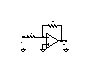
\includegraphics[scale=6]{schemi/invertente.eps}
		\end{center}
		\begin{multline}
			R_{in}=R \\
			R_{out}= ?? \\
			A_v=\frac{Vout}{Vin}=\frac{R_f}{R}
		\end{multline}	
	
	\subsubsection*{Tensione di offset}
	Le tensione di offset $V_{OS}$ è una tensione che causa un'uscita non nulla in presenza di un ingresso nullo. 
	Ad ingresso nullo si ha come uscita:
	\begin{align*}
		V_{O_{(in=0)}}= \left ( 1+\frac{R_f}{R} \right ) V_{OS}
	\end{align*}
	Questa equazione vale sia per la configurazione invertente che per quella non invertente.
	
	La tensione ottenuta, per sovrapposizione degli effetti, va a sommarsi al segnale in uscita. Questo va a influire sulla massima tensione in uscita dall'operazionale. 
	Il valore massimo che può assumere $V_{OS}$ viene fornito dal testo, ma in valore assoluto, perché il segno è casuale e varia da esemplare a esemplare del componente.
	Per tenere conto della tensione di offset, è sufficiente considerare un intervallo di variazione, ovvero scrivere:
	\begin{align*}
		V_O= A \cdot V_{IN} \pm V_{O_{(in=0)}} 
	\end{align*}
	
	In un solo caso è possibile ignorare del tutto l'effetto della tensione di offset: se all'ingresso dell'operazionale è presente un condensatore. Infatti il condensatore blocca le tensioni continue, ed essendo la tensione di offset proprio una tensione continua, impedisce che questa influisca nell'uscita. Questo però impedisce all'amplificatore di amplificare la continua, e nel caso sia necessario farlo, dovranno essere utilizzati altri mezzi per rendere l'offset trascurabile, mezzi che comunque non saranno presenti nel compito.
	
	\subsubsection*{Correnti di offset}
	Le correnti di offset sono quelle minime correnti che entrano negli ingressi dell'operazionale reale. Principalmente sono dovute alla tecnologia con cui è realizzato il componente. L'influenza di tali correnti si riscontra nell'uscita, similmente alla tensione di offset.
	
	Se il circuito è protetto con una resistenza $R_P$ in serie al morsetto non invertente e il valore di $R_P$ è:
	\begin{align*}
		R_P=\frac{R \cdot R_f}{R + R_f}
	\end{align*}
	ovvero il parallelo tra $R$ e $R_f$, allora il contributo sulla tensione di uscita delle correnti di offset è:
	\begin{equation}
		V_O=-I_{OS}R_f
	\end{equation}
	
	Se il circuito è sprovvisto della resistenza di protezione, occorre considerare il contributo di $I_{B2}$ come:
	\begin{equation}
		I_{B2}=I_B-\frac{I_{OS}}{2}
	\end{equation}
	mentre il contributo sulla tensione d'uscita sarà dato da:
	\begin{equation}
		V_O=I_{B2}R_f
	\end{equation}
	
	Ovviamente i contributi sulle tensioni d'uscita di entrambi i casi andranno sommati alla tensione d'uscita di segnale, avendo quindi:
	\begin{align*}
		V_O=A \cdot V_{IN} \pm contributo correnti.
	\end{align*}
	
	\subsubsection*{Massima ampiezza del segnale in ingresso affinché l'uscita sia lineare}
	L'ampiezza massima del segnale in uscita è limitata dallo slew-rate, come detto prima. L'ampiezza diminuisce al crescere della frequenza. Noi dobbiamo sapere qual è la massima ampiezza raggiungibile nella nostra banda di frequenze, quindi è necessario conoscere la pulsazione di taglio superiore del circuito, $\omega_{BF}$.\newline
	A questo punto, utilizziamo la seguente equazione:
	\begin{equation}
		V_{O_{max}}=\frac{SR}{\omega_{BF}}
	\end{equation}
	Ora è facile notare che la massima ampiezza del segnale in ingresso perché non ci siano problemi di non linearità è data da
	\begin{equation}
		V_{i_{max}}=\frac{V_{O_{max}}}{A_F}
	\end{equation}
	Nel caso di più stadi in cascata, se essi sono disaccoppiati ($R_{OUT1} \ll R_{IN2}$), allora il guadagno per cui bisogna dividere la tensione massima in uscita è il prodotto dei guadagni dei singoli stadi.
\end{document}
